%%%%%%%%%%%%%%%%%%%%%%%%%%%%%%%%%%%%%%%%%%%%%%%%%%%%%%%%%%%%%%%%%%%%%%%%%%%%%
%%%                                 FORM                                  %%%
%%%%%%%%%%%%%%%%%%%%%%%%%%%%%%%%%%%%%%%%%%%%%%%%%%%%%%%%%%%%%%%%%%%%%%%%%%%%%
\subsubsection{Form}
\label{sec:uiform}
\index{FORM@\FORM}
\index{FORM@\FORM!ui\_manager form}
A form is a Qt dialog window
that contains vertically and horizontally aligned form items
and a button bar. Each form item, except
  \STDWINDOW, \LOGWINDOW, \SEPARATOR, \VOID{} and \STRETCH,
must reference a previously declared
  \FOLDER, \FIELDGROUP
, \PLUGIN, \UNIPLOT, \LISTPLOT, \PLOTTHREED, \IMAGE
, \LIST, \LINEPLOT, \PLOTTWOD, \TEXTWINDOW, \NAVIGATOR
, \THERMO, \TIMETABLE{} or \TABLE{}. \\

\vspace{1cm}
Form items also are called {\bfseries CONTAINER ELEMENT}.\index{CONTAINER@container element}
See \nameref{dia:uiformcontainerelement} on page \pageref{dia:uiformcontainerelement}. \\

\input{diagrams/ui_form_list}

\label{uimanagerformhorizontallist}
\input{diagrams/ui_form_vertical_list}
\input{diagrams/ui_form_horizontal_list}
\input{diagrams/ui_form_container_options}

\index{SB@\SB!abbreviation|see{\SCROLLBARS}}
\index{NS@\NS!abbreviation|see{\NOSCROLLBARS}}
\index{PW@\PW!abbreviation|see{\PANEDWINDOW}}
\index{NP@\NP!abbreviation|see{\NOPANEDWINDOW}}

\index{SCROLLBARS@\SCROLLBARS!ui\_manager container option}
\index{ALWAYS@\ALWAYS!ui\_manager container scrollbars option}
\index{HORIZONTAL@\HORIZONTAL!ui\_manager container scrollbars option}
\index{VERTICAL@\VERTICAL!ui\_manager container scrollbars option}
\index{NO\_SCROLLBARS@\NOSCROLLBARS!ui\_manager container option}
\index{PANEDWINDOW@\PANEDWINDOW!ui\_manager container option}
\index{NO\_PANEDWINDOW@\NOPANEDWINDOW!ui\_manager container option}
\index{JUSTIFY@\JUSTIFY!ui\_manager container option}
\index{FRAME@\FRAME!ui\_manager container option}
\index{HELPTEXT@\HELPTEXT!ui\_manager container option}
\begin{tabularx}{\textwidth}{l|X}
item\_option   & description \\
\hline
\SCROLLBARS    & The container will have vertical and/or horizontal scroll bars. \newline
                 {\begin{tabular}{l|l|l}
                 options        & horizontal & vertical \\
                 \hline
                  & as needed & as needed \\
                 \ALWAYS & always & always \\
                 \HORIZONTAL & as needed & never \\
                 \HORIZONTAL{} \ALWAYS & always & as needed \\
                 \VERTICAL & never & as needed \\
                 \VERTICAL{} \ALWAYS & as needed & always \\
                 \end{tabular}} \\
\NOSCROLLBARS  & The container has no scroll bars.\\
\PANEDWINDOW   & The container will have a scrollable window separator (paned window).\\
\NOPANEDWINDOW & The container has no scrollable window separator (no paned window).\\
\JUSTIFY       & The rows or columns of the fieldgroups in the container are justified (aligned).\\
{\bfseries string}   & Display this string along with \FRAME. Has no effect without \FRAME. \\
\FRAME         & Display a frame around the container. \\
\HELPTEXT      & This text appears in the statusbar (or as a tooltip) as soon as the mouse-pointer is over this container.
\end{tabularx}

\input{diagrams/ui_form_container_element}

\index{STD\_WINDOW@\STDWINDOW!ui\_manager container element}
\index{LOG\_WINDOW@\LOGWINDOW!ui\_manager container element}
\index{SEPARATOR@\SEPARATOR!ui\_manager container element}
\index{TEXT\_WINDOW@\TEXTWINDOW!ui\_manager container element}
\index{VOID@\VOID!ui\_manager container element}
\index{STRETCH@\STRETCH!ui\_manager container element}
\begin{tabularx}{\textwidth}{l|X}
container element   & description \\
\hline
\STDWINDOW          & Standard window.\\
\LOGWINDOW          & Log window.\\
\SEPARATOR          & Separator line.\\
\VOID{} (n)         & an empty space of n pixels \\
\STRETCH{} (n)      & define a stretch factor of n.
                      The container is expanded here if additional space is available.
                      A higher stretch factor takes more of the available space. \\
\end{tabularx}

\input{diagrams/ui_form_element_identifier}

\newpage
All form items which are within a second pair of parentheses are placed horizontally, the others
vertically within the form. This is explained in the following
figure:
\vspace{1cm}

\begin{figure}[H]\label{fig:formItemArrangement}
  \begin{center}
    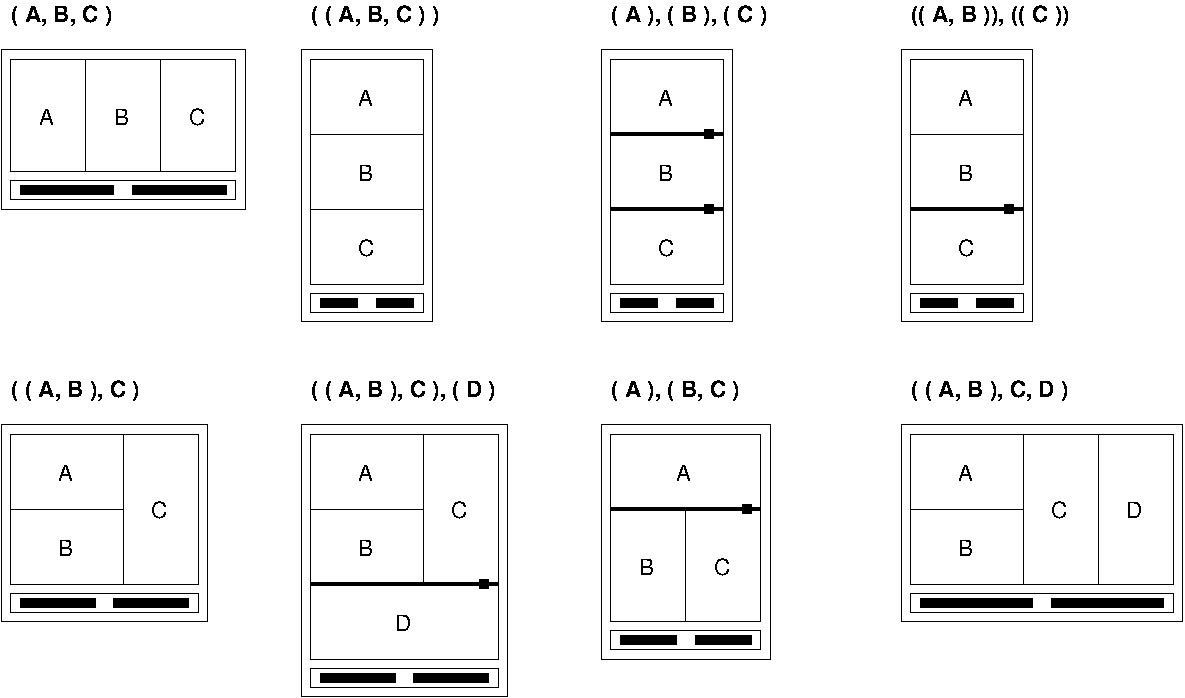
\includegraphics[width=\linewidth]{xfig/sntx_ui_form_comb}
  \end{center}
  \caption{FORM item arrangement examples}
\end{figure}

\newpage
The forms appearance can be changed with the following options:

\input{diagrams/ui_form_option_list}

\index{MAIN@\MAIN!ui\_manager form option}
\index{APP\_MODAL@\APPMODAL!ui\_manager form option}
\index{HIDDEN@\HIDDEN!ui\_manager form option}
\index{SCROLLBARS@\SCROLLBARS!ui\_manager form option}
\index{NO\_SCROLLBARS@\NOSCROLLBARS!ui\_manager form option}
\index{PANEDWINDOW@\PANEDWINDOW!ui\_manager form option}
\index{NO\_PANEDWINDOW@\NOPANEDWINDOW!ui\_manager form option}
%%(not implemented in intens4) \index{HELPTEXT@\HELPTEXT!ui\_manager form option}
\index{HIDE\_CYCLE@\HIDECYCLE!ui\_manager form option}
\index{HELPKEY@\HELPKEY!ui\_manager form option}
\index{BUTTONS@\BUTTONS!ui\_manager form option}
%%(not implemented in intens-qt) \index{JUSTIFY@\JUSTIFY!ui\_manager form option}
\index{FUNC@\FUNC!ui\_manager form option}
\index{CLOSE\_BUTTON@\CLOSEBUTTON!ui\_manager form option}
\index{EXPAND@\EXPAND!ui\_manager form option}
\begin{tabularx}{\textwidth}{l|X}
option                & description \\
\hline
\verb+string+         & defines the name of the window\\
\MAIN                 & places this form in the main window.\\
\APPMODAL             & opens the window modal.\\
\HIDDEN               & No menu entry will be created for this form.
                        You have to use the \MAP{} \FORM{} command to map this
                        form on the screen
                        (see section \nameref{sec:fudescription} on page \pageref{key:map_form}). \\
                      & When you create a menu entry for this form, you don't need this option
                        (see section \nameref{sec:uimenu} on page \pageref{key:menu_form}). \\
\SCROLLBARS           & The form has vertical and horizontal scroll bars
                        as needed. This is the default layout.\\
\NOSCROLLBARS         & The form has no scroll bars.\\
\PANEDWINDOW          & The fieldgroups will have a scrollable window separator.\\
\NOPANEDWINDOW        & The fieldgroups will not have a scrollable window separator.\\
%%(not implemented in intens-qt) \JUSTIFY              & The form will be justified.\\
\HIDECYCLE            & The button to change the datapool \CYCLE{} is not created.\\
\HELPKEY              & A help button is created that references a page in the help file.
                        (see section \nameref{sec:helpfile} on page \pageref{sec:helpfile})\\
\label{key:helpkey}
\BUTTONS              & Limits the number of buttons on the same action bar line and creates additional lines if needed. \\
%%(not implemented in intens4) \HELPTEXT             & This text appears in the statusbar (or as a tooltip) as soon as the mouse-pointer is over this form. \\
\USERGROUPS           & A list of usergroups or the identifier of a predefined group of usergroups.
                        (see section \nameref{sec:usergroups} on page \pageref{sec:usergroups})\\
\FUNC                 & Defines the function that will be called when a form is opened, closed or activated.
                        (see also section \nameref{sec:functions} on page \pageref{sec:functions})\\
\CLOSEBUTTON          & Do not show a {\bfseries Close} button at the bottom of the \FORM. \\
\EXPAND               & Adapt the size of the \FORM{} when it is opened and when an element in it is shown or hidden. \\
\end{tabularx}
